\subsection{Planning for Complex Task Solving}
\label{subsec-planning}
Prompting with ICL and CoT is a conceptually simple yet general approach to solving various tasks. 
However, this approach struggles with complex tasks like mathematical reasoning~\cite{Qian-2022-arXiv-limitations} and multi-hop question answering~\cite{Ning-arxiv-2023-ChatGPT}.
As an enhanced approach, prompt-based planning has been proposed to break down complex tasks into smaller sub-tasks and generate a plan of actions to accomplish the task.

\subsubsection{The Overall Framework}

\begin{figure}[t]
    \centering
    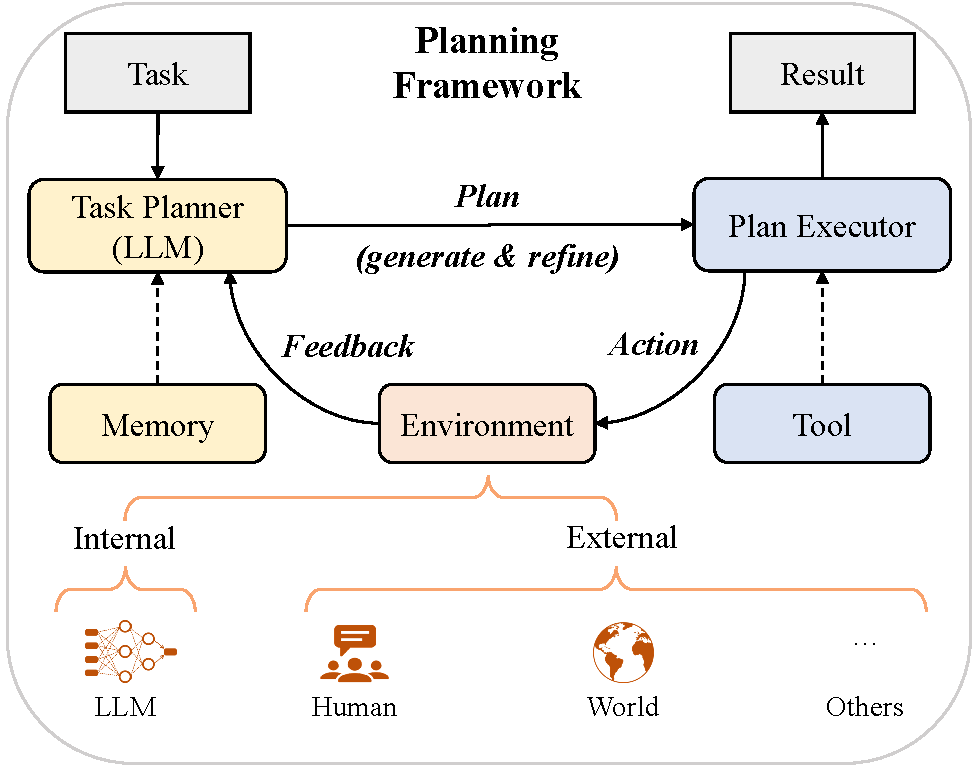
\includegraphics[width=\linewidth]{images/planning-v3.pdf}
    \caption{An illustration of the formulation for prompt based planning by LLMs for solving complex tasks.}
    \label{fig:planning}
\end{figure}

In this part, we first formulate the general planning paradigm of LLMs for solving complex tasks, which is illustrated in Figure~\ref{fig:planning}.

In this paradigm, there are typically three components: \emph{task planner}, \emph{plan executor}, and \emph{environment}\footnote{
Despite the similarity with RL, our formulation decouples the planning and execution phases, whereas in RL, they are typically interleaved in the agent.
This paradigm is defined in a general yet slightly loose way, and it mainly aims to help readers understand the key idea underlying the planning approaches of LLMs.
}.
Specifically, task planner, which is played by LLMs, aims to generate the whole plan to solve a target task.
The plan can be presented in various forms, \eg an action sequence in the form of natural language~\cite{Zhou-arxiv-2022-Least} or an executable program written in programming language~\cite{Gao-arxiv-2022-PAL}.
The LLM-based task planner can be enhanced with the memory mechanism for plan storage and retrieval, which is helpful for long-horizon tasks.
Then, plan executor is responsible for executing the actions in the plan.
It can be implemented by models like LLMs for textual tasks~\cite{Wang-arXiv-2023-Plan} or by tools like code interpreters for coding tasks~\cite{Shinn-2023-arXiv-Reflexion}.
Furthermore, environment refers to where the plan executor carries out the actions, which can be set differently according to specific tasks, \eg the LLM itself~\cite{Yao-2023-arXiv-tree} or an external virtual world like Minecraft~\cite{Wang-2023-arXiv-voyager}.
It provides \textit{feedback} about the execution result of the action to the task planner, either in the form of natural language~\cite{Shinn-2023-arXiv-Reflexion} or from other multimodal signals~\cite{Lu-2023-arXiv-multimodal}.

For solving a complex task, the task planner first needs to clearly understand the task goal and generate a reasonable plan based on the reasoning of LLMs (See Section~\ref{sec:plan-gen}).
Then, the plan executor acts according to the plan in the environment, and the environment will produce feedback for the task planner (See Section~\ref{sec:feedback}).
The task planner can further incorporate the feedback obtained from the environment to refine its initial plan and iteratively perform the above process to get better results as the task solution (See Section~\ref{sec:plan-refine}).


\subsubsection{Plan Generation}
\label{sec:plan-gen}
Plan generation focuses on directly generating action sequences by prompting LLMs.
Based on the format of the generated plans, existing work can be divided into two groups: text-based and code-based approaches. 

\paratitle{Text-based Approaches.}
It is straightforward for LLMs to generate plans in the form of natural language.
In this approach, LLMs are prompted to generate a sequence of actions for the plan executor to perform and solve the complex task.
For example, Plan-and-Solve~\cite{Wang-arXiv-2023-Plan} adds explicit instructions like ``\texttt{devise a plan}'' to directly prompt the LLM for planning in a zero-shot manner, while Self-planning~\cite{Jiang-arXiv-2023-Self} and DECOMP~\cite{Khot-2022-arXiv-Decomposed} add demonstrations in the prompt to guide the LLM to devise a plan through ICL.
Following this way, some work further considers incorporating extra tools or models when planning. 
For example, ToolFormer~\cite{Schick-arxiv-2023-Toolformer} first annotates a pre-training corpus with potential API calls using LLMs, and then fine-tunes LLMs on it,  so that LLMs can learn when and how to call APIs and incorporate the results returned by APIs during generation.
HuggingGPT~\cite{Shen-2023-arXiv-Hugginggpt} introduces the models available in HuggingFace and regards LLMs as the controller to select suitable models based on their descriptions and aggregate their results as the final solution.

\paratitle{Code-based Approaches.}
Although text-based approaches sound intuitive, they cannot guarantee faithful execution of the plan, which may lead to failure even when the plan is sound. 
To address this issue, code-based approaches have been proposed to generate more verifiable plans in the form of executable code in  programming languages, \eg Python or PDDL.
In this way, LLMs are first prompted to generate the program and then utilize a deterministic solver to execute it.
For example, Faithful CoT~\cite{Lyu-arxiv-2023-Faithful} and PAL~\cite{Gao-arxiv-2022-PAL} decompose a reasoning task into two stages: at the first stage, the LLM generates a plan conditioned on the query; at the second stage, a deterministic solver executes the plan to derive the final answer. 
Furthermore, code-based approaches can be applied to embodied agents in a similar way. 
For example, PROGPROMPT~\cite{Singh-arxiv-2022-ProgPrompt} and LLM+P~\cite{Liu-2023-arXiv-LLM+P} first utilize LLMs to generate plans in the form of python functions or PDDL files, and then leverage a virtual agent or classical planner to solve the problem according to the code-based plans.

\subsubsection{Feedback Acquisition}
\label{sec:feedback}
After executing the generated plan, the environment would produce the feedback signal to the LLM-based task planner, which can be used to refine its initial plan for better results.
In existing work, there are typically two sources of feedback from the environment, depending on their relationship with the LLM-based task planner: internal (\ie the LLM itself) and external (\eg tools or virtual worlds) feedback.

\paratitle{Internal Feedback.}
The LLM itself can be utilized as a feedback provider.
One straightforward way is to directly evaluate the quality of the generated plans through prompting.
For example, RAP~\cite{Hao-2023-arXiv-reasoning} evaluate the likelihood that each candidate plan can lead to task success, while Tree of Thoughts~\cite{Yao-2023-arXiv-tree} proposes to vote across plans by making comparisons between them.
Further, LLMs can provide feedback based on the intermediate results from the plan executor.
For example, Reflexion~\cite{Shinn-2023-arXiv-Reflexion} utilizes LLMs to transform sparse result signals (\eg success or failure) into concrete {text-based feedback (\eg ``\emph{You should recommend comedies that the user mentions in the query instead of horror movies}'') and stores this feedback in long-term memory for future planning.}


\paratitle{External Feedback.}
In addition to LLMs, external objects can also provide feedback signals.
For example, tools like code interpreters are widely used in programming tasks to provide real-time error messages~\cite{Shinn-2023-arXiv-Reflexion}, models like stable diffusion~\cite{Rombach-2022-CVPR-high} can be used in multimodal tasks to provide visual perception~\cite{Lu-2023-arXiv-multimodal}, and {virtual worlds} like Minecraft can provide immersive experiences~\cite{Wang-2023-arXiv-voyager}.
Besides, some work (\eg Generative Agents~\cite{Park-arxiv-2023-Generative}) explores multi-agent collaboration in simulated environments, where each agent receives feedback not only from interaction with the environment but also from communication with other agents.

\subsubsection{Plan Refinement}
\label{sec:plan-refine}
With access to feedback from the environment, the task planner can accordingly refine its current plan and iteratively go through the ``\emph{planning -- execution -- refinement}'' loop for better results.
In this part, we summarizes three major refinement approaches in existing work. 

\paratitle{Reasoning.}
The feedback data from the environment may not be directly suitable to be utilized by LLMs for plan refinement, \eg containing irrelevant information or taking a non-language form.
To solve this, some work adds the explicit reasoning process to extract critical information from feedback~\cite{Yao-2022-arXiv-react, Chen-2023-arXiv-chatcot}.
For example, React~\cite{Yao-2022-arXiv-react} prompts LLMs with demonstrations to generate reasoning traces over feedback.
It has been widely used in autonomous agent projects, such as AutoGPT~\cite{AutoGPT}, which can automatically reason over the observed feedback to revise the initial plan for solving various user requests.
However, these approaches typically fix the order of reasoning and planning.
To support flexible switching between the two processes for better performance, ChatCoT~\cite{Chen-2023-arXiv-chatcot} further unifies the tool-augmented reasoning process into a multi-turn conversation between the LLM-based task planner and the tool-based environment.

\paratitle{Backtracking.}
Early methods mainly consider planning forward actions while maintaining the existing plan, thus likely leading to local optimal plans based on a short-term evaluation.
To solve this, Tree of Thoughts~\cite{Yao-2023-arXiv-tree} allows backtracking with search algorithms like breadth-first and depth-first search to make global planning.
It refines the plan step by step by backtracking to the last state in the initial plan and choosing the next unexplored action.
Furthermore, some studies~\cite{Wang-2023-arXiv-describe, Lu-2023-arXiv-multimodal} utilize feedback signals to revise the entire plan.
For example, DEPS~\cite{Wang-2023-arXiv-describe} selects a better plan according to feedback signals, while TIP~\cite{Lu-2023-arXiv-multimodal} adds feedback signals to prompts for the LLM-based planner to revise each step in the initial plan.

\paratitle{Memorization.}
In order to handle long-horizon tasks, it has become a key approach to aid plan refinement with \emph{long-term memory} in addition to utilizing the \emph{short-term memory} of LLMs through ICL.
For example, Reflexion~\cite{Shinn-2023-arXiv-Reflexion} stores the feedback from self-reflection into the memory, so previous feedback can be retrieved for plan refinement.
Generative Agents~\cite{Park-arxiv-2023-Generative} designs the memory stream mechanism as the core component of agents for action planning and reflection.
Further, the skill library mechanism~\cite{Wang-2023-arXiv-voyager, Sun-2023-arXiv-adaplanner} is proposed to store successful plans in the library, which can be reused and synthesized as complex plans for novel tasks.
To implement the long-term memory mechanism, tools like vector databases (\eg milvus~\cite{Wang-2021-ICDM-Milvus}) can be used to encode plans or feedbacks into high-dimensional vectors for efficient storage and retrieval at a large scale.
MemoryBank~\cite{Zhong-2023-arxiv-MemoryBank} further proposes the memory updating mechanism to allow memory forgetting and strengthening following the Ebbinghaus Forgetting Curve theory.


